% Options for packages loaded elsewhere
\PassOptionsToPackage{unicode}{hyperref}
\PassOptionsToPackage{hyphens}{url}
%
\documentclass[
  12pt,
  a4paper,
  oneside]{report}
\usepackage{lmodern}
\usepackage{setspace}
\usepackage{amssymb,amsmath}
\usepackage{ifxetex,ifluatex}
\ifnum 0\ifxetex 1\fi\ifluatex 1\fi=0 % if pdftex
  \usepackage[T1]{fontenc}
  \usepackage[utf8]{inputenc}
  \usepackage{textcomp} % provide euro and other symbols
\else % if luatex or xetex
  \usepackage{unicode-math}
  \defaultfontfeatures{Scale=MatchLowercase}
  \defaultfontfeatures[\rmfamily]{Ligatures=TeX,Scale=1}
  \setmainfont[]{Lato}
\fi
% Use upquote if available, for straight quotes in verbatim environments
\IfFileExists{upquote.sty}{\usepackage{upquote}}{}
\IfFileExists{microtype.sty}{% use microtype if available
  \usepackage[]{microtype}
  \UseMicrotypeSet[protrusion]{basicmath} % disable protrusion for tt fonts
}{}
\makeatletter
\@ifundefined{KOMAClassName}{% if non-KOMA class
  \IfFileExists{parskip.sty}{%
    \usepackage{parskip}
  }{% else
    \setlength{\parindent}{0pt}
    \setlength{\parskip}{6pt plus 2pt minus 1pt}}
}{% if KOMA class
  \KOMAoptions{parskip=half}}
\makeatother
\usepackage{xcolor}
\IfFileExists{xurl.sty}{\usepackage{xurl}}{} % add URL line breaks if available
\IfFileExists{bookmark.sty}{\usepackage{bookmark}}{\usepackage{hyperref}}
\hypersetup{
  pdftitle={Comment caractériser et inférer les interactions dans les communautés écologiques ?},
  pdfkeywords={Network inference, Network Analysis, JDSM},
  hidelinks,
  pdfcreator={LaTeX via pandoc}}
\urlstyle{same} % disable monospaced font for URLs
\usepackage[left = 2cm,right = 2cm,top = 2cm,bottom = 2cm]{geometry}
\usepackage{longtable,booktabs}
% Correct order of tables after \paragraph or \subparagraph
\usepackage{etoolbox}
\makeatletter
\patchcmd\longtable{\par}{\if@noskipsec\mbox{}\fi\par}{}{}
\makeatother
% Allow footnotes in longtable head/foot
\IfFileExists{footnotehyper.sty}{\usepackage{footnotehyper}}{\usepackage{footnote}}
\makesavenoteenv{longtable}
\usepackage{graphicx,grffile}
\makeatletter
\def\maxwidth{\ifdim\Gin@nat@width>\linewidth\linewidth\else\Gin@nat@width\fi}
\def\maxheight{\ifdim\Gin@nat@height>\textheight\textheight\else\Gin@nat@height\fi}
\makeatother
% Scale images if necessary, so that they will not overflow the page
% margins by default, and it is still possible to overwrite the defaults
% using explicit options in \includegraphics[width, height, ...]{}
\setkeys{Gin}{width=\maxwidth,height=\maxheight,keepaspectratio}
% Set default figure placement to htbp
\makeatletter
\def\fps@figure{htbp}
\makeatother
\setlength{\emergencystretch}{3em} % prevent overfull lines
\providecommand{\tightlist}{%
  \setlength{\itemsep}{0pt}\setlength{\parskip}{0pt}}
\setcounter{secnumdepth}{-\maxdimen} % remove section numbering

%% pandoc-fignos: required package
\usepackage{cleveref}

%% pandoc-fignos: change cref names
\crefname{figure}{figure}{figs.}

%% pandoc-eqnos: disable brackets around cleveref numbers
\creflabelformat{equation}{#2#1#3}

%% pandoc-eqnos: change cref names
\crefname{equation}{équation}{eqs.}

%% pandoc-tablenos: change cref names
\crefname{table}{tableau}{tables}

\title{Comment caractériser et inférer les interactions dans les communautés
écologiques ?}
\usepackage{etoolbox}
\makeatletter
\providecommand{\subtitle}[1]{% add subtitle to \maketitle
  \apptocmd{\@title}{\par {\large #1 \par}}{}{}
}
\makeatother
\subtitle{UE Analyse Bibliographique}
\date{}

\begin{document}
\maketitle

{
\setcounter{tocdepth}{2}
\tableofcontents
}
\setstretch{1.5}
\hypertarget{introduction}{%
\chapter{Introduction}\label{introduction}}

Les interactions sont un des éléments clés de voute de la structure des
communautés biologiques. Ainsi, dès le début de l'écologie moderne, les
interactions sont apparues comme l'un des deux éléments importants dans
la lutte pour le plus apte (Darwin 2004). Ainsi, à des échelles
temporelles et spatiales réduites, les interactions sont le principal
facteur de la biodiversité (Benton 2009), c'est l'hypothèse de la
\emph{Reine Rouge} (Van Valen 1973).

Cependant, les connaissances sur les interactions intraspécifiques et
interspécifiques sont encore aujourd'hui très lacunaires
(Morales-Castilla et al. 2015 ; Rosado et al. 2016). Ce manque de
connaissance peut s'expliquer par le fait qu'il est actuellement
impossible d'observer les interactions entre les espèces. Par exemple,
un écosystème avec seulement sept espèces différentes peut donner lieu à
l'observation de 42 directes interactions et plus de 13 000 interactions
indirectes (Morales-Castilla et al. 2015).

La caractérisation et l'inférence des interactions entre les espèces
peuvent sembler alors une tâche qui n'a que peut d'intérêt au vu de sa
complexité. Toutefois, il existe des preuves dans la littérature que les
interactions peuvent affecter l'aire de répartition et la
co-distribution des espèces à des échelles spatiales locales, voire
continentales. De plus, les interactions pourraient également moduler
les réponses biologiques des espèces face aux changements
environnementaux (Morales-Castilla et al. 2015). De plus en plus de
recherches se penchent ainsi sur la prédiction du fonctionnement des
écosystèmes face aux changements globaux. C'est pourquoi la prédiction
des interactions entre les espèces d'un même écosystème devient un enjeu
majeur en écologie des communautés (Montoya \& Raffaelli 2010).

\hypertarget{les-interactions-en-uxe9cologie}{%
\chapter{Les interactions en
écologie}\label{les-interactions-en-uxe9cologie}}

\hypertarget{diffuxe9rentes-interactions}{%
\section{Différentes interactions}\label{diffuxe9rentes-interactions}}

Une interaction pourrait être définie comme l'action d'une première
espèce sur une seconde. De fait, il existe plusieurs façons de décrire
les interactions en écologie : les interactions peuvent varier selon
leur type (antagoniste ou facilitatrice), leur forcent (faible ou forte)
ainsi que leur symétrie (symétriques ou asymétriques) et leur mode
d'action (direct ou indirect) (Wootton 1994 ; Morales-Castilla et al.
2015). Cette définition n'englobe pas une échelle écologique précise :
les interactions peuvent être observées au niveau des individus, de
populations ou bien encore d'espèces.

Dans un premier temps, nous nous intéresserons aux interactions
directes, puis aux interactions indirectes.

\hypertarget{les-interactions-directes}{%
\section{Les interactions directes}\label{les-interactions-directes}}

Historiquement, le premier type d'interaction étudié a été les
interactions directes grâce à l'observation de réseaux trophique, il y a
plus d'un siècle (Dunne 2006). Une interaction directe est définie comme
une interaction physique entre deux individus : un donneur et un
receveur. (Wootton 1994). Dans les années 70, c'est l'étude des
interactions hôtes-parasites qui a connu un rapide gain d'intérêt.
Enfin, au début des années 2000, ce sont les réseaux mutualistes qui ont
été mis sur le devant de la scène par les chercheurs (Poisot et al.
2019). C'est pourquoi traditionnellement les réseaux écologiques sont
subdivisés dans ces trois catégories citées au-dessus (Ings et al.
2009). Toutefois, il est possible de définir plus d'interactions
directes comme le montre le \cref{tbl:1}.

\begin{longtable}[]{@{}ll@{}}
\caption{Exemple des différents types d'interaction qu'il est possible
de rencontrer en écologie. L'espèce qui effectue l'interaction est dans
la partie gauche de la parenthèse et celle qui subit l'interaction est
sur la partie droite de la parenthèse. L'effet de l'interaction est
représenté par un symbole. Adapté de Morales-Castilla et al. (2015).
\label{tbl:1}}\tabularnewline
\toprule
Type d'interaction et nature de l'effet & Exemple
Biologique\tabularnewline
\midrule
\endfirsthead
\toprule
Type d'interaction et nature de l'effet & Exemple
Biologique\tabularnewline
\midrule
\endhead
Mutualisme (+, +) & Fleurs et insectes polinisateurs\tabularnewline
Prédation / Parasitisme (+, -) & Lions et gnous\tabularnewline
Commensalisme (+, 0) & Crevettes nettoyeuses et les
muraenidae\tabularnewline
Amensalime (0, -) & Piétinement des pelouses par l'Homme\tabularnewline
\bottomrule
\end{longtable}

\hypertarget{les-interactions-indirectes}{%
\section{Les interactions
indirectes}\label{les-interactions-indirectes}}

Les interactions indirectes forment la seconde grande classe
d'interaction qui structurent les communautés écologiques. Les
interactions indirectes peuvent être définies comme l'effet d'un
individu ou d'une espèce émetteur d'une interaction sur une autre
(receveur) par la médiation d'un troisième transmetteur. Wootton (1994)
démontre que les interactions indirectes peuvent se propager de deux
manières différentes : par une chaîne d'interaction ou par une
modification des interactions.

Une chaîne d'interaction est décrite comme l'interaction d'une espèce A
sur une autre espèce B via une espèce transmettrice. Par exemple, une
espèce peut réduire l'abondance de sa proie, réduisant ainsi la base
alimentaire des autres consommateurs de la proie (Wootton 1994).

La modification des interactions se produit lorsque le changement
d'abondance d'une espèce A peut indirectement affecter l'abondance d'une
espèce B en modifiant l'interaction entre l'espèce B et une espèce C.
Wootton (1994) donnent l'exemple suivant : l'augmentation de la densité
de la végétation peut augmenter indirectement l'abondance d'une espèce
prédatée en lui permettant de se cacher de ses prédateurs, réduisant
ainsi l'intensité de l'interaction proie-prédateur.

Menge (1995) a proposé sept grands types d'interactions indirectes
\cref{fig:interactions_menge} :

\begin{itemize}
\tightlist
\item
  Prédation clé de voute : interaction observée lorsque l'abondance d'un
  prédateur augmente indirectement l'abondance des concurrents de sa
  proie par la consommation de ladite proie ;
\item
  Cascade trophique : augmentation de l'abondance d'une espèce causée
  par le contrôle de son prédateur immédiat par un autre prédateur ;
\item
  Exploitation concurrentielle : réduction de l'abondance d'un
  consommateur résultant de la réduction de l'abondance sa proie par une
  autre espèce de consommateur ;
\item
  Compétition : réduction de l'abondance d'une espèce résultant de
  l'augmentation de l'abondance d'une deuxième espèce qui augmente la
  prédation par un prédateur commun ;
\item
  Mutualisme indirect : Changements positivement corrélés de l'abondance
  de deux espèces résultant de la prédation de chacune sur la proie
  principale de l'autre ;
\item
  Commensalisme indirect : résulte du fait qu'une des deux espèces de
  prédateurs dans un schéma de mutualisme indirect à un régime
  alimentaire plus large et se nourrit également de la proie principale
  de l'autre espèce de prédateur dans le schéma de mutualiste indirect ;
\item
  Facilitation d'habitat : un organisme améliore indirectement l'habitat
  d'un deuxième en modifiant l'abondance d'une troisième espèce.
\end{itemize}

\begin{figure}
\hypertarget{fig:interactions_menge}{%
\centering
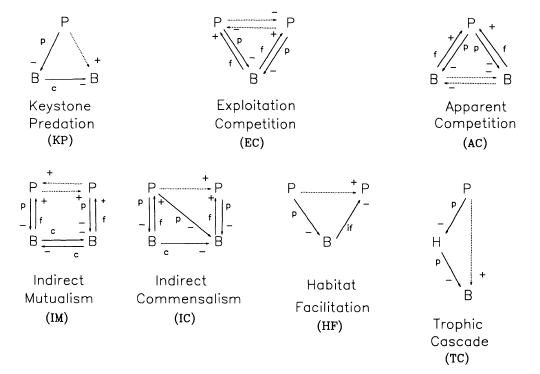
\includegraphics{figures/indirect_interaction_menge.png}
\caption{Schéma des différents types d'effets indirects. P, prédateur ;
H, herbivore ; B, espèce basale. Les flèches pleines représentent les
effets directs, les flèches en pointillés représentent les effets
indirects. +, effet positif ; -, effet négatif. p, prédation ; c,
compétition d'interférence ; f, apport de nourriture ; if, inhibition de
la prise alimentaire. Adapté de Menge
(1995).}\label{fig:interactions_menge}
}
\end{figure}

\hypertarget{caractuxe9ristiques-des-interactions}{%
\chapter{Caractéristiques des
interactions}\label{caractuxe9ristiques-des-interactions}}

\hypertarget{ruxe9seau-dinteraction-et-thuxe9orie-des-graphes}{%
\section{Réseau d'interaction et théorie des
graphes}\label{ruxe9seau-dinteraction-et-thuxe9orie-des-graphes}}

Les réseaux écologiques d'interactions peuvent être représentés à l'aide
de graphes. Les graphes sont des constructions mathématiques constituées
de deux ensembles : les noeuds et les arêtes qui représentent les
connexions entre des paires de noeuds (Dale \& Fortin 2010). Ces outils
mathématiques facililent la représentation des interactions, chaque
noeud étant une espèce et chaque arrête représentant une interaction.
Les arrêtes peuvent être orienté ou non. Si le graphe est orientés,
alors la direction de l'interaction entre l'espèce emetrice et receveuse
de l'interaction est indiquée par l'arrête sous la forme d'une flêche
(Dunne 2006 ; Dale \& Fortin 2010 ; Delmas et al. 2018).

L'utilisation de graphes en écologie permet d'utiliser un ensemble
d'outils développés par les mathématiciens pour mieux comprendre les
réseaux complexes. Il existe ainsi des outils permettant de décrire
comment les espèces interagissent au sein d'une communauté, quel est le
rôle de chaque espèce dans la communauté (Delmas et al. 2018) etc. Aussi
pour ce travail, il ne sera question dans les prochains paragraphes que
de quelques-uns des outils permettant de décrire comment les espèces
interagissent entre elles.

Une des propriétés basiques d'un graphe découle de sa définition : le
nombre de noeuds. Dans le cas d'un réseau écologique, chaque noeud est
associé à une espèce (Dunne 2006 ; Delmas et al. 2018). \(S\) représente
ainsi la riche spécifique d'une communauté. De même, il est possible de
définir le degré \(deg\) comme le nombre d'arrête pour un noeud et \(L\)
comme le nombre d'arrêtes tout un réseau écologique. C'est ainsi qu'il
est possible de déduire la densité d'un réseau écologique en appliquant
le rapport \(\frac{L}{S}\) qui indique le nombre de liens qui est
attendu pour une espèce prise au hasard. Toutefois, la mesure de la
densité n'est pas un indicateur satisfaisant, en effet il ne représente
pas l'ensemble des liens possible dans un réseau d'interaction. C'est
alors que Martinez (1992) proposa une autre mesure la connectance. La
formule de la connectance \(C = \frac{L}{m}\) varie selon le type de
réseau considéré : si les espèces peuvent interagir avec elles-mêmes,
alors \(m = S^2\) dans le cas contraire \(m = (S - 1)^2\). La propriété
de la connectance est importante pour les réseaux écologiques, car elle
permet de donner des indications quant à la fragilité du réseau.

La distribution des degrés est la mesure qui donne la probabilité qu'une
espèce ait \(k\) interaction. Cette mesure se calcule de la manière
suivante : \(P(k) = N_k / S\) avec \(N_k\) le nombre de noeuds ayant
\(k\) arrêtes. La distribution de degrés d'un graphe est une mesure
permettant l'identification des espèces clés de voute potentielles
(Dunne 2006). De plus, les degrés d'un graphe peuvent, dans le cas d'un
graphe orienté être décomposés en arrête entrantes et sortantes d'un
noeud. Ainsi, il est possible de déterminer d'autres mesures comme le
nombre de prédateurs et le nombre d'espèces prédites (Delmas et al.
2018).

Les réseaux d'interactions peuvent être également décomposés en
sous-graphes plus petits : les motifs. Les motifs sont des assemblages
de trois noeuds, il en existe 13 différents pour les graphes orientés.
La fréquence de ces différents motifs donne aux biologistes des
informations sur la structure des réseaux d'interactions, puisque
certains motifs sont présents à une fréquence différente de celle du
hasard. Les motifs sont considérés comme la brique de construction
élémentaire d'un réseau d'interaction. L'étude des motifs se trouve
particulièrement efficace pour étudier les processus déterminant
l'assemblage et le désassemblage des communautés ou bien encore pour
étudier le rôle trophique d'une espèce et lier ce lien avec la stabilité
du réseau d'interaction (Dunne 2006 ; Delmas et al. 2018).

Un dernier outil de mesure de la structure des réseaux d'interaction
issue de la théorie des graphes est l'intervalité. Pour calculer
l'intervalité d'un réseau d'interaction biologique, il faut trouver un
trait commun à tous les noeuds pour lequel il est possible d'ordonner
tous les noeuds. Cela peut être fait pour les réseaux trophiques à
l'aide de la taille ou de la masse moyenne d'un individu. Les réseaux
d'interactions qui peuvent être entièrement décrit par une seule
dimension (un trait) sans qu'il y ait d'ex aequo sont dits
``intervalles'' (Delmas et al. 2018). Les réseaux trophiques étudiés par
Eklöf et al. (2013) d'une taille inférieur à 250 espèces se sont montrés
être ``intervalles'', ainsi les réseaux trophiques sont considérés comme
quasi-intervalles, puisqu'un nombre réduit de dimensions permet
d'expliquer leur structure. L'intervalité offre une perspective
intéressante à l'utilisation de certains outils de réduction de la
dimensionnalité pour expliquer la structure des réseaux d'interaction en
écologie à l'instar de l'ACP utilisée par Vermaat et al. (2009).

Toutefois, ces mesures d'analyse de la structure des réseaux
d'interaction ont une limite importante. L'hypothèse sous-jacente est la
suivante : si deux espèces dans un graphe sont reliées entre elles par
une arrête, alors ces deux espèces interagissent forcément ensemble.
Hors les interactions entre espèces sont des entités dynamiques, elles
varient en fonction de l'espace et du temps et d'effets comportementaux
ainsi que stochastiques (Poisot et al. 2014). C'est ainsi que Poisot et
al. (2016) propose d'un changement de paradigme en ne se posant plus la
question si deux espèces interagissent, mais plutôt de savoir quelle est
la probabilité qu'elles interagit. Dans ce même article, les auteurs
proposent de redéfinir l'ensemble de ces métriques pour prendre en
compte la nature stochastique des interactions en écologie.

\hypertarget{pruxe9dire-les-interactions}{%
\chapter{Prédire les interactions}\label{pruxe9dire-les-interactions}}

En écologie trophique il existe une boîte à outils de méthodes pour
observer des interactions entre des proies et des prédateurs grâce à un
certain nombre d'outils. Ces outils passent par de l'observation
directe, de l'analyse de contenus stomacaux, les mesures d'isotopes
stables, des contaminants ou bien encore des méthodes statistiques
(Majdi et al. 2018). Mais ces méthodes ne permettent pas de faire
d'inférence par rapport aux autres types d'interactions.

Ces dernières années, un ensemble de nouvelles méthodes statiques ont
été développées pour estimer la distribution spatiale et/ou temporelle à
l'aide de données de co-occurrence ou d'abondance, ce sont les
\emph{Spatial Distribution Models} (\emph{SDM}). Ces méthodes peuvent
être utilisées pour analyser simultanément la distribution corrélée de
plusieurs espèces (Thorson et al. 2016). Ces nouvelles méthodes ont
également l'avantage de pouvoir prendre en compte les interactions entre
les espèces et éventuellement de les estimer.

Dans les prochains paragraphes, il sera question de quelques une de ces
méthodes : \emph{Latent Variable Model}, \emph{Hierarchical Modelling of
Species Communities}, \emph{Gaussian copula graphical models} et
quelques methodes de Machine Learning. Enfin, dans une dernière partie,
il s'agira d'avoir un regard critique sur les données de co-occurrence
et leurs apports pour prédire les interactions entre espèces.

\hypertarget{latent-variable-models}{%
\section{\texorpdfstring{\emph{Latent Variable
Models}}{Latent Variable Models}}\label{latent-variable-models}}

Le but des \emph{Latent Variable Models} (\emph{LVM}) est de décrire les
corrélations entre l'abondance des taxons en fonction de variables
explicatives, ce genre de modèle fait parti d'une plus grande famille de
modèles en écologie des communautés, nommés les \emph{Joint species
distribution models}. Les \emph{LVM} sont des extensions des
\emph{Generalized Linear Model} (\emph{GLM}) et ils incluent une forme
d'effet aléatoire pour permettre de prendre en compte les corrélations
d'abondance entre les espèces (\cref{eq:eq1}). Dans le cas des
\emph{LVM}, l'effet aléatoire est inclus grâce à des variables latentes
: c'est-à-dire des variables non mesurées par l'expérimentateur (Warton
et al. 2015).

\begin{equation}g(m_{ij}) = \alpha_i + \beta_{0j} + x_i'\beta_j + z_i'\lambda_j\label{eq:eq1}\end{equation}

\(g()\) est la fonction de lien comme dans un GLM, qui relie la moyenne
estimée au prédicteur linéaire. \(m_{ij}\) est l'abondance moyenne de
l'espèce \(j\) au site \(i\). \(\alpha_{i}\) est un terme facultatif qui
s'ajuste en fonction de l'abondance relative ou de la richesse totale du
site pour modéliser de l'abondance relative plutôt que sur l'abondance
absolue.\(x'\) est la transposé des données d'abondance pour chaque
espèce \(j\), \(\beta_{0j}\) est l'ordonné à l'origine et \(\beta_j\)
est un vecteur de coefficient de régression estimé à partir des
variables explicatives. Enfin \(\lambda_j\) est un facteur de charge lié
aux variables latentes \(z_i\). Cette variable latente est traitée comme
un facteur aléatoire, comme l'abondance en assumant que
\(y_{ij}|z_i \sim F(m_{ij}, \phi_j)\) et \(z_i \sim N(0,1)\). Ainsi, la
distribution de l'abondance connaissant la valeur de la variable latente
suit une loi de probabilité caractérisée par une moyenne (\(m_{ij}\)) et
un paramètre de dispersion (\(\phi_j\)). La difficulté d'estimer un tel
modèle réside dans l'estimation des variables latentes et des facteurs
de charges, car non observée. Il faut alors avoir recourt à des priors
ou de l'inférence bayésienne. Mais son intérêt réside également dans le
fait que cette méthode permet de réduire le nombre de coefficients de
corrélation à estimer lorsqu'elle est comparée à un \emph{Generalized
Linear Mixed Model} multivarié. Le temps de calcul d'un \emph{LVM} est
d'un dixième de celui d'un \emph{Generalized Linear Mixed Model} pour un
jeu de donnée de co-occurrence à 65 colonnes et 75 lignes (Warton et al.
2015).

Les \emph{LVM} permettent d'estimer les corrélations entre les espèces
après avoir contrôlé l'effet de variables environnementales, mais
également d'utiliser les variables latentes comme des axes d'ordination
et bien entendu faire de l'inférence multivariée pour de la projection.
Les \emph{LVM} sont également intéressantes pour inférer les
interactions entre les espèces, puisque les variables latentes peuvent
être interprétées comme des variables comprenant les interactions entre
les espèces au sein d'une même communauté.

Rapidement un package R est sorti pour permettre aux écologistes de
mettre facilement en oeuvre les \emph{LVM} comme \emph{boreal} d'après
les travaux de Hui (2016).

\hypertarget{hierarchical-modelling-of-species-communities}{%
\section{\texorpdfstring{\emph{Hierarchical Modelling of Species
Communities}}{Hierarchical Modelling of Species Communities}}\label{hierarchical-modelling-of-species-communities}}

Quelques années après le papier de Warton et al. (2015), Ovaskainen et
al. (2017) proposèrent une extension des \emph{JSDM} nommés
\emph{Hierarchical Modelling of Species Communities} (\emph{HMSC}). Ce
nouveau cadre statistique propose d'intégrer des données d'occurrence ou
d'abondance, de données environnementales, le contexte spatio-temporel
du plan d'échantillonnage, des données de trait et de phylogénie
\cref{fig:hmsc_summary}.

\begin{figure}
\hypertarget{fig:hmsc_summary}{%
\centering
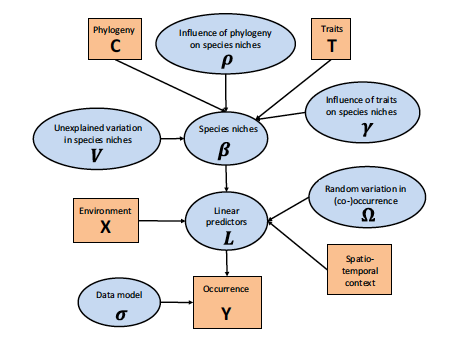
\includegraphics{figures/hmsc_summary.png}
\caption{Schéma conceptuel du cadre de modélisation statique
\emph{HMSC}. Les rectangles orange font référence aux données que peut
entrer dans le modèle l'utilisateur et les ellipses bleues font
référence aux paramètres qu'il est possible d'observer. Adapté de
Ovaskainen et al. (2017).}\label{fig:hmsc_summary}
}
\end{figure}

Pour fonctionner, les \emph{HMSC} ont besoin au minimum de données
d'abondance (ou de co-occurrence), ainsi que des données
environnementales (matrices \(X\) et \(Y\) \cref{fig:hmsc_summary}).

Ce genre de modèles peut répondre à un large éventail de questions comme
quelle part de la variance de l'abondance des espèces est due aux
filtres environnementaux, aux interactions biotiques et aux processus
aléatoires ? Quelles sont les structures des réseaux d'interaction entre
les espèces ? Ou bien encore est-ce que la présence de certaines espèces
indique la présence d'autres ? (Ovaskainen et al. 2017).

L'inférence d'interaction est rendue possible grâce à l'estimation de de
la matrice d'association \(\Omega\) (\cref{fig:hmsc_summary}). Cette
matrice estime si deux espèces ont une probabilité d'occurrence
supérieure à celle du hasard. Pour \(m\) espèce, cette matrice
\(\Omega\) a \(m(m+1)/2\) paramètres à estimer, ce qui rend la tâche
complexe lorsque \(m\) est suffisamment grand. Pour contourner ce
problème, Ovaskainen et al. (2017) utilisent une méthode dérivée des
\emph{LVM}, ils utilisent les facteurs de charges associés aux variables
latentes pour estimer la matrice \(\Omega\). Bien que les auteurs soient
d'accord sur le fait que ces facteurs de charge n'expriment pas
directement des interactions au sens écologique du terme, ils sont
utiles pour révéler des configurations où deux espèces sont présentes en
même temps plus souvent que le hasard ne peut l'expliquer.

Pour utiliser ce cadre de modélisation, un package R a été développé
pour mettre en place les analyses de type \emph{HMSC} (Tikhonov et al.
2019). Ainsi, ce type d'analyse a été mis en place sur les herbiers de
zoostère\footnote{Un des milieux biogènes qui sera au coeur de mon
  stage.} (\emph{Zostera marina}) par Stark et al. (2018). Ils ont ainsi
pu mettre en évidence de signaux forts de co-occurrence d'espèces
antagonistes entre différents sites, ce qui leur a permis de supposer de
fortes interactions biotiques qui pourraient se traduire par exemple,
par de la compétition entre les espèces herbivores pour l'accès à la
production primaire. Les auteurs font également l'hypothèse que la
structuration des communautés de \emph{Zostera marina} peut également
traduire un effet prioritaire\footnote{Effet que peut avoir une espèce
  particulière sur le développement d'une communauté, car elle s'est
  installée plus tôt sur le site.} important sur les herbiers plus
récents.

\hypertarget{gaussian-copula-graphical-models}{%
\section{\texorpdfstring{\emph{Gaussian Copula Graphical
Models}}{Gaussian Copula Graphical Models}}\label{gaussian-copula-graphical-models}}

Pour estimer l'interaction entre espèces Popovic et al. (2019) proposent
l'utilisation d'un nouveau cadre de modélisation statique :
\emph{Gaussian Copula Graphical Models} (\emph{GCGM}). Ce nouveau type
de modèle couple une distribution multivariée gaussienne à un autre type
de distribution marginale à choisir en fonction du type de donnée :
distribution binomiale pour des données de présence/absence,
distribution de Poisson pour des données d'abondance, etc. Cette
combinaison permet d'accéder aux corrélations de co-occurrence d'espèce
pour tout type de données et l'utilisation d'une copule gaussienne
permet d'utiliser des modèles graphiques gaussiens pour estimer les
liens d'interactions entre les différentes espèces. Ainsi, ce nouveau
type de méthode est capable d'utiliser tout type de données d'occurrence
utilisée en écologie. Sa grande flexibilité en fait une des forces de ce
nouvel outil. Pour faciliter son utilisation, les auteurs de cet article
ont mis à disposition un package R. Grâce au \emph{GCGM} il est possible
d'obtenir des graphes non orientés qui permettent de voir les relations
entre chaque espèce. Il est alors possible d'observer les interactions
directe et indirecte entre les différentes espèces. De plus, l'obtention
de graphes non orientés permet d'utiliser certaines mesures de la
théorie des graphes pour permettre des interprétations plus larges sur
la structure du réseau écologique. Toutefois, quelques précautions sont
à prendre avec l'analyse de cette méthode : les espèces qui semblent
interagir entre elles peuvent répondre de la même façon à une variable
environnementale non mesurée et l'absence d'interaction peut également
être un artefact lié à un problème d'échantillonnage.

\hypertarget{machine-learning}{%
\section{\texorpdfstring{\emph{Machine
Learning}}{Machine Learning}}\label{machine-learning}}

Depuis quelques années, les écologues se sont emparés des méthodes de
\emph{Machine Learning} pour répondre à de vaste question. A partir de
catalogue d'interactions il est possible de déterminer pour de nouvelles
espèces, lesquelles sont susceptible d'interagir entre elles (Beauchesne
et al. 2017; Desjardins-Proulx et al. 2017 ) . L'algorithme retenu dans
les deux cas a été celui des plus proches voisins (\emph{KNN}). Bien que
l'implémentation et la création du catalogue d'interaction permettant
l'inférerance soit de nature différente, les auteurs de ces deux
articles notent de très belles performances pour prédire les
interactions trophiques. Desjardins-Proulx et al. (2017) montrent que
leur algorithme est capable de prédire correctement la proie d'un
prédateur plus de 50\% du temps parmi un ensemble de plus de 800 proies
possible. L'algorithme de Beauchesne et al. (2017) fait mieux en
arrivant à prédire correctement les interactions entre 80\% et presque
100\% du temps. La différence de précision peut être en partie expliquée
par la construction des catalogues d'interactions.

Desjardins-Proulx et al. (2017) ont également utilisé dans leur article
un algorithme d'apprentissage supervisé, les \emph{Random Forest}.
Utilisant uniquement trois traits : la masse et deux variables portant
sur les relations phylogénétiques, ils ont montré qu'il était possible
de prédire correctement plus de 95\% du temps les interactions et
non-interactions dans un réseau trophique.

Cette dernière approche a ouvert la piste à d'autres chercheurs qui se
sont intéressés à prédire les interactions entre les plantes et les
pollinisateurs (Pichler et al. 2019). Dans leur article, les auteurs
montrent par exemple que les algorithmes de \emph{Random Forest} ou de
\emph{Deep Neural Network} sont capables de prédire correctement grâce
aux traits près de 90\% des interactions et surpassent d'autres méthodes
statistiques plus classiques comme les \emph{GLM}. De plus, ces
algorithmes permettent aussi d'inférer quels sont les traits qui
régulent les interactions entre les plantes et les oiseaux mouches sans
avoir eu à faire d'hypothèses à priori sur le fonctionnement du système.
Les auteurs mettent l'accent sur le fait que les algorithmes de
\emph{Machine Learning} offrent beaucoup d'avantages par rapport aux
modèles de régression. Au vu du potentiel de ces algorithmes, les
auteurs encouragent leur utilisation pour prédire les interactions dans
d'autres types de réseaux d'interactions.

\hypertarget{bibliographie}{%
\chapter*{Bibliographie}\label{bibliographie}}
\addcontentsline{toc}{chapter}{Bibliographie}

\hypertarget{refs}{}
\leavevmode\hypertarget{ref-Beauchesne_2017b}{}%
\textbf{Beauchesne et al.} (2017). Thinking outside the box - Predicting
biotic interactions in data-poor environments. \emph{Vie et Milieu.}
66:333--42.

\leavevmode\hypertarget{ref-Benton_2009}{}%
\textbf{Benton}. (2009). The red queen and the court jester: Species
diversity and the role of biotic and abiotic factors through time.
\emph{Science.} American Association for the Advancement of Science
(AAAS); 323:728--32.

\leavevmode\hypertarget{ref-Dale_2010}{}%
\textbf{Dale \& Fortin}. (2010). From graphs to spatial graphs.
\emph{Annual Review of Ecology, Evolution, and Systematics.} Annual
Reviews; 41:21--38.

\leavevmode\hypertarget{ref-Darwin_2004}{}%
\textbf{Darwin}. (2004). On the origin of species, 1859. Routledge;

\leavevmode\hypertarget{ref-Delmas_2018}{}%
\textbf{Delmas et al.} (2018). Analysing ecological networks of species
interactions. \emph{Biological Reviews.} Wiley; 94:16--36.

\leavevmode\hypertarget{ref-Desjardins-Proulx_2017}{}%
\textbf{Desjardins-Proulx et al.} (2017). Ecological interactions and
the Netflix problem. \emph{PeerJ.} 5:e3644.

\leavevmode\hypertarget{ref-Dunne_2006}{}%
\textbf{Dunne}. (2006). The network structure of food webs. In: Dunne,
Mercedes, eds. \emph{Ecological networks: Linking structure to dynamics
in food webs.} Oxford University Press, pp. 27--86.

\leavevmode\hypertarget{ref-Eklof_2013}{}%
\textbf{Eklöf et al.} (2013). The dimensionality of ecological networks.
Dunne, ed. \emph{Ecology Letters.} Wiley; 16:577--83.

\leavevmode\hypertarget{ref-Hui_2016}{}%
\textbf{Hui}. (2016). Boral -- bayesian ordination and regression
analysis of multivariate abundance data in r. \emph{Methods in Ecology
and Evolution.} 7:744--50.

\leavevmode\hypertarget{ref-Ings_2009}{}%
\textbf{Ings et al.} (2009). Review: Ecological networks - beyond food
webs. \emph{Journal of Animal Ecology.} Wiley; 78:253--69.

\leavevmode\hypertarget{ref-Majdi_2018}{}%
\textbf{Majdi et al.} (2018). There's no harm in having too much: A
comprehensive toolbox of methods in trophic ecology. \emph{Food Webs.}
17:e00100.

\leavevmode\hypertarget{ref-Martinez_1992}{}%
\textbf{Martinez}. (1992). Constant connectance in community food webs.
\emph{The American Naturalist.} University of Chicago Press;
139:1208--18.

\leavevmode\hypertarget{ref-Menge_1995}{}%
\textbf{Menge}. (1995). Indirect effects in marine rocky intertidal
interaction webs: Patterns and importance. \emph{Ecological Monographs.}
Wiley; 65:21--74.

\leavevmode\hypertarget{ref-Montoya_2010}{}%
\textbf{Montoya \& Raffaelli}. (2010). Climate change, biotic
interactions and ecosystem services. \emph{Philosophical Transactions of
the Royal Society B: Biological Sciences.} The Royal Society;
365:2013--8.

\leavevmode\hypertarget{ref-Morales_Castilla_2015}{}%
\textbf{Morales-Castilla et al.} (2015). Inferring biotic interactions
from proxies. \emph{Trends in Ecology \& Evolution.} Elsevier BV;
30:347--56.

\leavevmode\hypertarget{ref-Ovaskainen_2017_procB}{}%
\textbf{Ovaskainen et al.} (2017). How are species interactions
structured in species-rich communities? A new method for analysing
time-series data. \emph{Proceedings of the Royal Society B: Biological
Sciences.} 284:20170768.

\leavevmode\hypertarget{ref-Pichler_2019}{}%
\textbf{Pichler et al.} (2019). Machine learning algorithms to infer
trait-matching and predict species interactions in ecological networks.
Carvalheiro, ed. \emph{Methods in Ecology and Evolution.} Wiley;

\leavevmode\hypertarget{ref-Poisot_2019}{}%
\textbf{Poisot et al.} (2019). Environmental biases in the study of
ecological networks at the planetary scale.

\leavevmode\hypertarget{ref-Poisot_2016}{}%
\textbf{Poisot et al.} (2016). The structure of probabilistic networks.
\emph{Methods in Ecology and Evolution.} 7:303--12.

\leavevmode\hypertarget{ref-Poisot_2014}{}%
\textbf{Poisot et al.} (2014). Beyond species: why ecological
interactions vary through space and time. \emph{Oikos.} Cold Spring
Harbor Laboratory Press; 124:243--51.

\leavevmode\hypertarget{ref-Popovic_2019}{}%
\textbf{Popovic et al.} (2019). Untangling direct species associations
from indirect mediator species effects with graphical models. Murrell,
ed. \emph{Methods in Ecology and Evolution.} Wiley; 10:1571--83.

\leavevmode\hypertarget{ref-Rosado_2016}{}%
\textbf{Rosado et al.} (2016). Eltonian shortfall due to the grinnellian
view: Functional ecology between the mismatch of niche concepts.
\emph{Ecography.} Wiley; 39:1034--41.

\leavevmode\hypertarget{ref-Stark_2018}{}%
\textbf{Stark et al.} (2018). Beyond a single patch: Local and regional
processes explain diversity patterns in a seagrass epifaunal
metacommunity. \emph{bioRxiv.}

\leavevmode\hypertarget{ref-Thorson_2016}{}%
\textbf{Thorson et al.} (2016). Joint dynamic species distribution
models: A tool for community ordination and spatio-temporal monitoring.
\emph{Global Ecology and Biogeography.} Wiley; 25:1144--58.

\leavevmode\hypertarget{ref-Tikhonov_2019}{}%
\textbf{Tikhonov et al.} (2019). Joint species distribution modelling
with hmsc-r. \emph{bioRxiv.} Cold Spring Harbor Laboratory;

\leavevmode\hypertarget{ref-Van_Valen_1973}{}%
\textbf{Van Valen}. (1973). A new evolutionary law. \emph{Evol Theory.}
1:1--30.

\leavevmode\hypertarget{ref-Vermaat_2009}{}%
\textbf{Vermaat et al.} (2009). Major dimensions in food-web structure
properties. \emph{Ecology.} Wiley; 90:278--82.

\leavevmode\hypertarget{ref-Warton_2015}{}%
\textbf{Warton et al.} (2015). So many variables: Joint modeling in
community ecology. \emph{Trends in Ecology \& Evolution.} Elsevier;
30:766--79.

\leavevmode\hypertarget{ref-Wootton_1994}{}%
\textbf{Wootton}. (1994). The nature and consequences of indirect
effects in ecological communities. \emph{Annual Review of Ecology and
Systematics.} Annual Reviews; 25:443--66.

\end{document}
